\section{Arquitectura del Sistema}

Esta sección describe los componentes principales del sistema, sus responsabilidades e interacciones, así como las tecnologías propuestas para su implementación.

\vspace{1cm}

\begin{figure}[H]
    \centering
    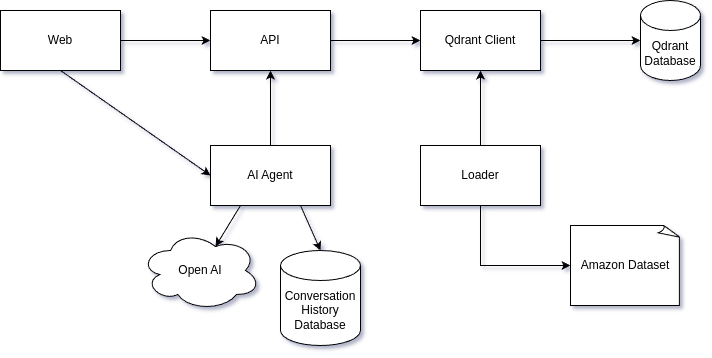
\includegraphics[width=0.8\textwidth]{architecture.png}
    \caption{Diagrama de alto nivel de la arquitectura del sistema.}
    \label{fig:system_architecture}
\end{figure}

\subsection{API}

Este componente constituye la capa de servicios que comunica el frontend con los distintos motores de búsqueda y recomendación. Incluye endpoints para listar productos (recibiendo parámetros de filtros y búsqueda) y para obtener información detallada de productos específicos.

\subsubsection{Implementación}

La API será implementada utilizando \href{https://fastapi.tiangolo.com/}{FastAPI}~\cite{FastAPI}, un framework moderno de Python que permite un desarrollo eficiente y robusto. FastAPI ofrece validación automática de datos mediante \href{https://docs.pydantic.dev/latest/}{Pydantic}~\cite{Pydantic}, tipado estático que reduce errores en tiempo de desarrollo, y generación automática de documentación con OpenAPI y Swagger UI. Esta documentación servirá como recurso valioso para la fase de desarrollo del frontend.

\subsection{Dataset}

Para la información de productos, se utilizará el conjunto de datos de Amazon disponible en \href{https://www.kaggle.com/datasets/lokeshparab/amazon-products-dataset/data?select=Amazon-Products.csv}{Kaggle}~\cite{Amazon}. Este conjunto de datos ofrece una amplia variedad de atributos por producto, incluyendo:

\begin{itemize}
    \item Título y descripción detallada
    \item Categorías y subcategorías
    \item Precio y disponibilidad
    \item Valoraciones y número de reseñas
    \item Imágenes de productos
    \item Especificaciones técnicas
\end{itemize}

La riqueza de estos atributos permitirá implementar las modalidades de búsqueda previamente mencionadas.
